\documentclass[10pt]{beamer}
\usepackage{etex}
\usepackage{multicol}
\usepackage{media9}
\usetheme[
%%% options passed to the outer theme
%    progressstyle=fixedCircCnt,   %either fixedCircCnt, movCircCnt, or corner
%    rotationcw,          % change the rotation direction from counter-clockwise to clockwise
%    shownavsym          % show the navigation symbols
  ]{AAUsimple}
  
% If you want to change the colors of the various elements in the theme, edit and uncomment the following lines
% Change the bar and sidebar colors:
%\setbeamercolor{AAUsimple}{fg=red!20,bg=red}
%\setbeamercolor{sidebar}{bg=red!20}
% Change the color of the structural elements:
%\setbeamercolor{structure}{fg=red}
% Change the frame title text color:
%\setbeamercolor{frametitle}{fg=blue}
% Change the normal text color background:
%\setbeamercolor{normal text}{fg=black,bg=gray!10}
% ... and you can of course change a lot more - see the beamer user manual.

\usepackage[utf8]{inputenc}
\usepackage[spanish]{babel}
\usepackage[T1]{fontenc}
% Or whatever. Note that the encoding and the font should match. If T1
% does not look nice, try deleting the line with the fontenc.
\usepackage{helvet}
\usepackage{graphics}
\usepackage{color}
\usepackage[all]{xy}


\usepackage{graphicx}
\graphicspath{ {AAUgraphics/} }

% colored hyperlinks
\newcommand{\chref}[2]{%
  \href{#1}{{\usebeamercolor[bg]{AAUsimple}#2}}%
}

\title{Diseño e implementación de una interfaz entre las bibliotecas OMPL y nD FMM \vspace{0.5cm}}

\subtitle{TRABAJO FIN DE GRADO}  % could also be a conference name

\date{13 de octubre de 2015}

\author{
Álvaro Muñoz Serrano
}

% - Give the names in the same order as they appear in the paper.
% - Use the \inst{?} command only if the authors have different
%   affiliation. See the beamer manual for an example

\institute[
%  {\includegraphics[scale=0.2]{aau_segl}}\\ %insert a company, department or university logo
%  Dept.\ of Electronic Systems\\
%  Aalborg University\\
%  Denmark
] % optional - is placed in the bottom of the sidebar on every slide
{% is placed on the bottom of the title page
 Departamento de Sistemas y Automática
  
  %there must be an empty line above this line - otherwise some unwanted space is added between the university and the country (I do not know why;( )
}

% specify a logo on the titlepage (you can specify additional logos an include them in 
% institute command below
\pgfdeclareimage[height=2.75cm]{titlepagelogo}{AAUgraphics/logocei.png} % placed on the title page
\titlegraphic{% is placed on the bottom of the title page
  \pgfuseimage{titlepagelogo}
%  \hspace{1cm}\pgfuseimage{titlepagelogo2}
}

\setcounter{tocdepth}{1}

\begin{document}
% the titlepage
{%\aauwavesbg%
\begin{frame}[plain,noframenumbering] % the plain option removes the header from the title page
  \titlepage
\end{frame}}
%%%%%%%%%%%%%%%%

% TOC
\begin{frame}{Índice}{}
\tableofcontents
\end{frame}
%%%%%%%%%%%%%%%%

\section{Motivación y objetivos}

\begin{frame}{Motivación}		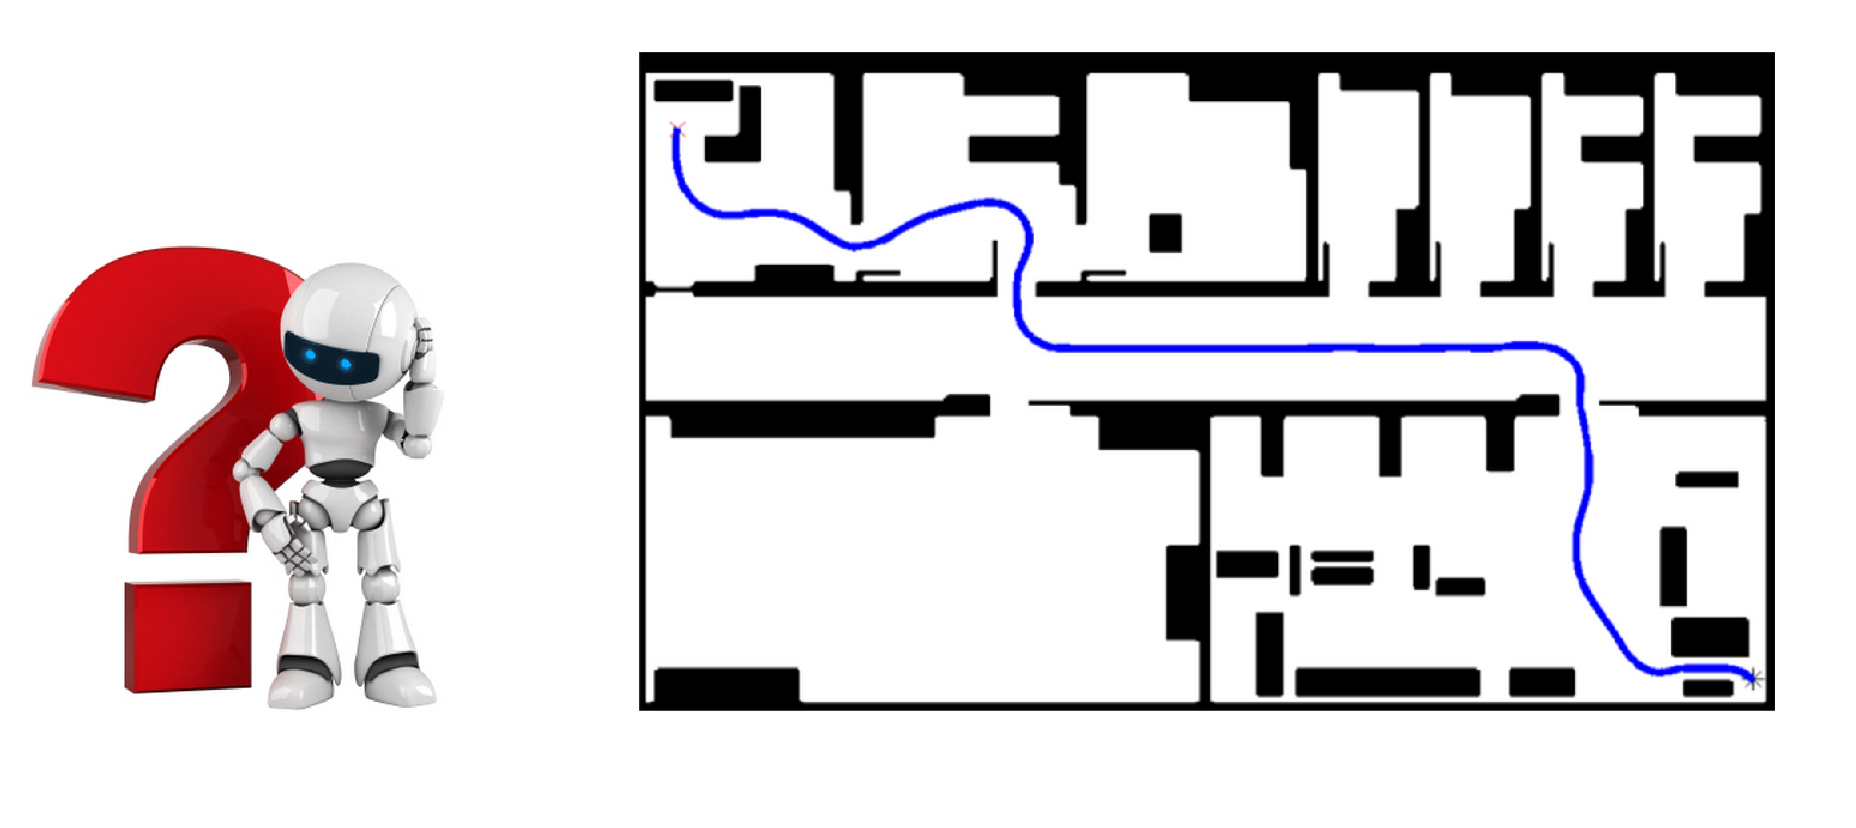
\includegraphics[width=\textwidth,height=0.8\textheight,keepaspectratio]{dudabot}
\end{frame}

\begin{frame}{Objetivos}
	\large nD FMM: n-Dimensional Fast Marching Methods
	\vspace{1cm}
	
	\large OMPL: Open Motion Planning Library
\end{frame}

\begin{frame}{Objetivos}
Crear una interfaz que permita complementar las funcionalidades que ofrecen ambas bibliotecas.
\vspace{0.3cm}
\begin{itemize}
	\item nD FMM
		\begin{itemize}
			\item Cargar entornos y robots 3D
			\item Aplicar orientación de los robots
			\item Visualizar resultados
		\end{itemize}
		\vspace{0.3cm}
	\item OMPL
		\begin{itemize}
			\item Utilizar algoritmos basados en Fast Marching
		\end{itemize}
\end{itemize}
\end{frame}

\section{Marco teórico}

\subsection{Planificación de movimientos}

\begin{frame}
	\textbf{OBJETIVO:} Trasladar un objeto de un lugar a otro sin colisionar con obstáculos.
	
	\begin{itemize}
		\item Métodos combinatorios		
		\item Métodos basados en muestreo aleatorio
		
	\end{itemize}		
\end{frame}

\begin{frame}\addtocounter{framenumber}{-1}
	\vspace{1.5cm}
	\textbf{OBJETIVO:} Trasladar un objeto de un lugar a otro sin colisionar con obstáculos.
	
	\begin{itemize}
		\item Métodos combinatorios		
		\item Métodos basados en muestreo aleatorio		
	\end{itemize}		
	\begin{center}
		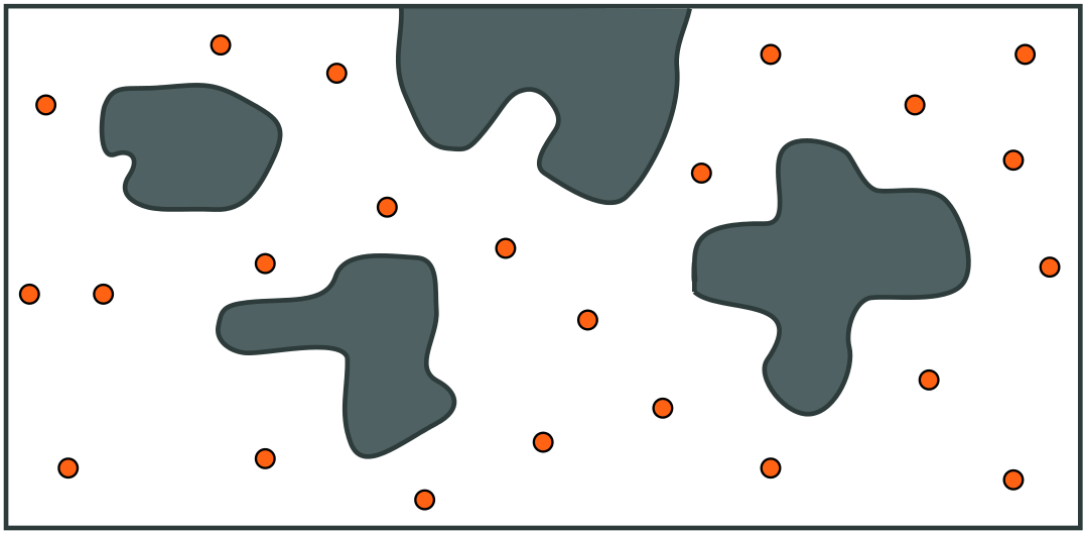
\includegraphics[width=0.5\textwidth,keepaspectratio]{prm_1}
	\end{center}
	
\end{frame}

\begin{frame}\addtocounter{framenumber}{-1}
	\vspace{1.5cm}
	\textbf{OBJETIVO:} Trasladar un objeto de un lugar a otro sin colisionar con obstáculos.
	\begin{itemize}
		\item Métodos combinatorios		
		\item Métodos basados en muestreo aleatorio		
	\end{itemize}		
	\begin{center}
		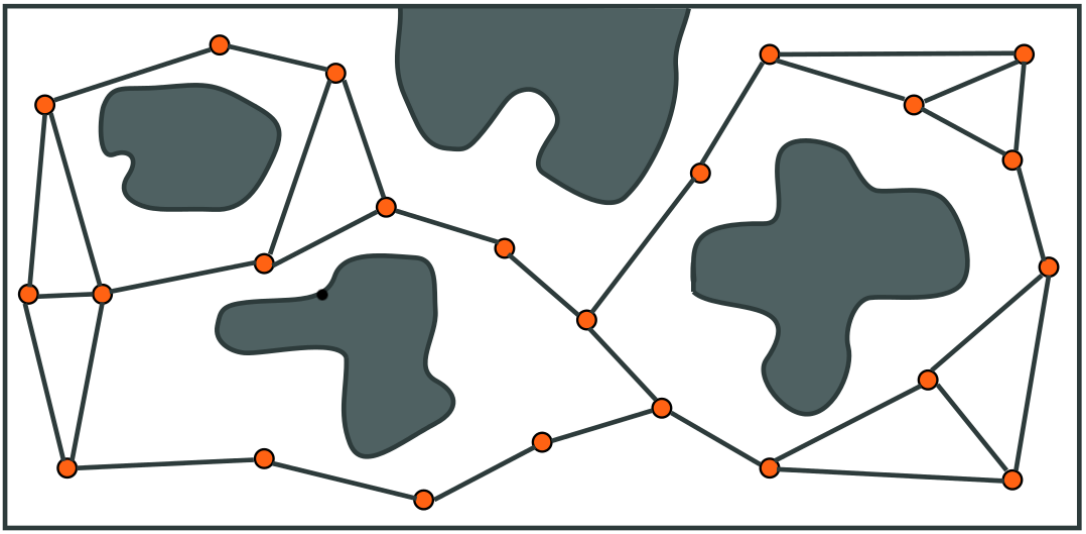
\includegraphics[width=0.5\textwidth,keepaspectratio]{prm_2}
	\end{center}
	
\end{frame}

\begin{frame}\addtocounter{framenumber}{-1}
	\vspace{1.5cm}
	\textbf{OBJETIVO:} Trasladar un objeto de un lugar a otro sin colisionar con obstáculos.
	
	\begin{itemize}
		\item Métodos combinatorios		
		\item Métodos basados en muestreo aleatorio		
	\end{itemize}		
	\begin{center}
		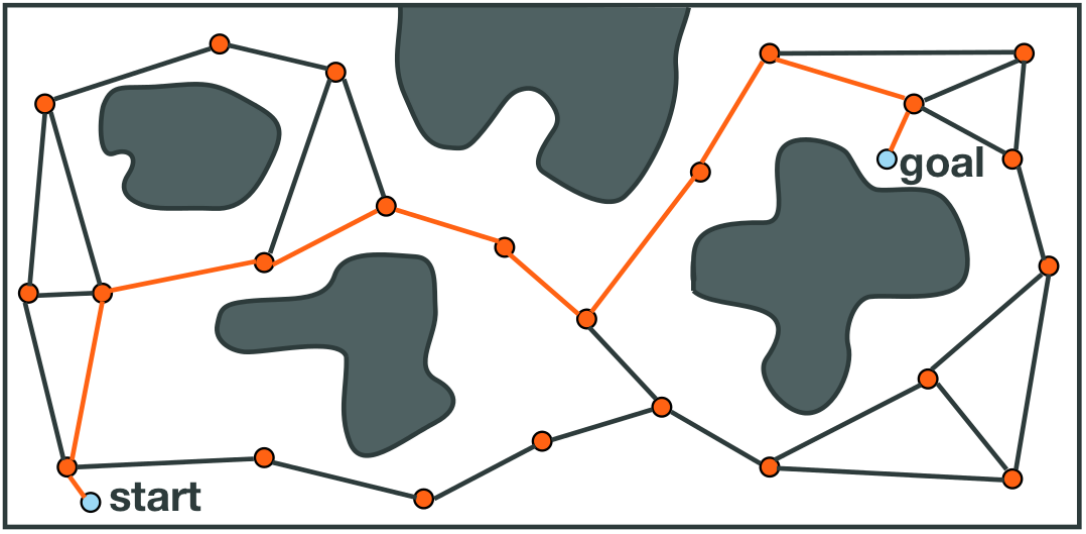
\includegraphics[width=0.5\textwidth,keepaspectratio]{prm_3}
	\end{center}
	
\end{frame}

\begin{frame}{Fast Marching Method}
\begin{itemize}
	\item El FMM es un método numérico que modeliza el comportamiento de una onda.
	\item Se basa en la ecuación Eikonal
\end{itemize}

	\begin{equation}
	1=F(x)\left| \nabla T(x) \right| 
	\end{equation}
	
\end{frame}

\subsubsection{FMM fotos}
\begin{frame}{Fast Marching Method}
	\begin{center}	
	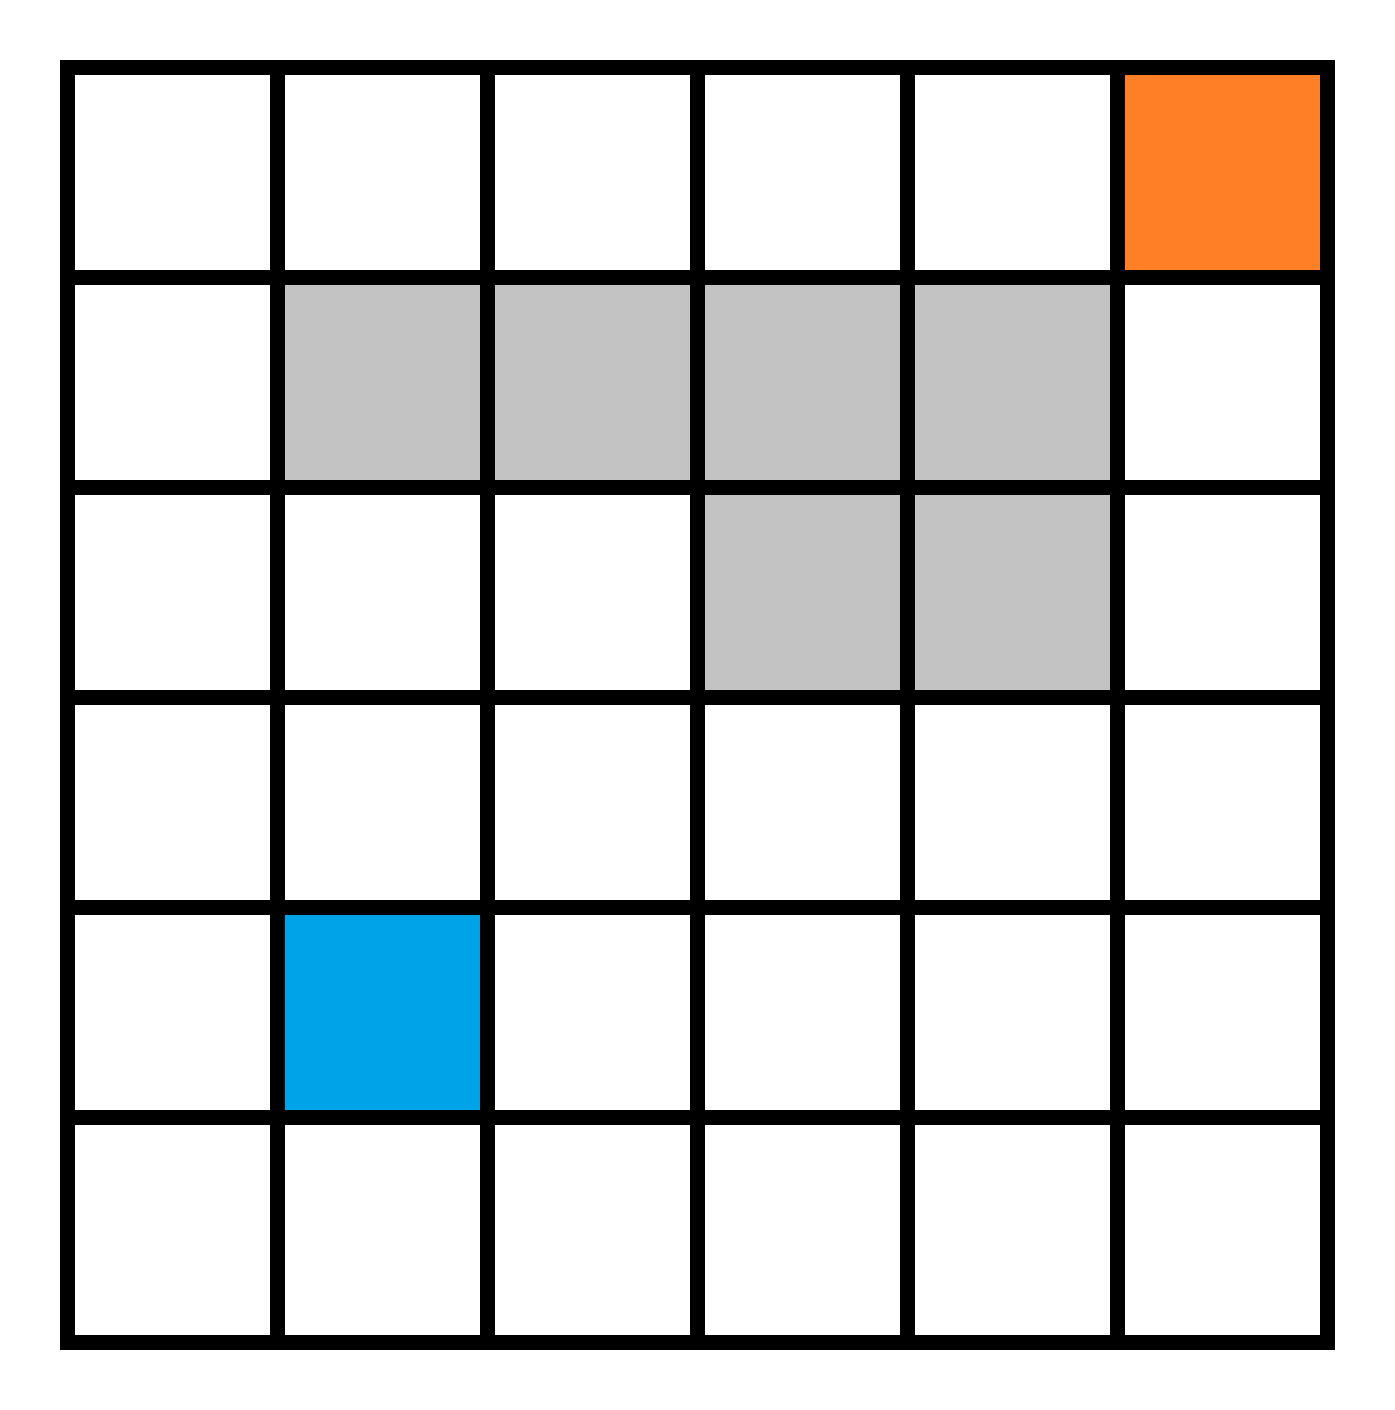
\includegraphics[width=\textwidth,height=0.8\textheight,keepaspectratio]{/FMM/grid0}	
	\end{center}
\end{frame}
\begin{frame}{Fast Marching Method}\addtocounter{framenumber}{-1}
	\begin{center}	
	\includegraphics[width=\textwidth,height=0.8\textheight,keepaspectratio]{/FMM/grid1}	
	\end{center}
\end{frame}
\begin{frame}{Fast Marching Method}\addtocounter{framenumber}{-1}
	\begin{center}	
	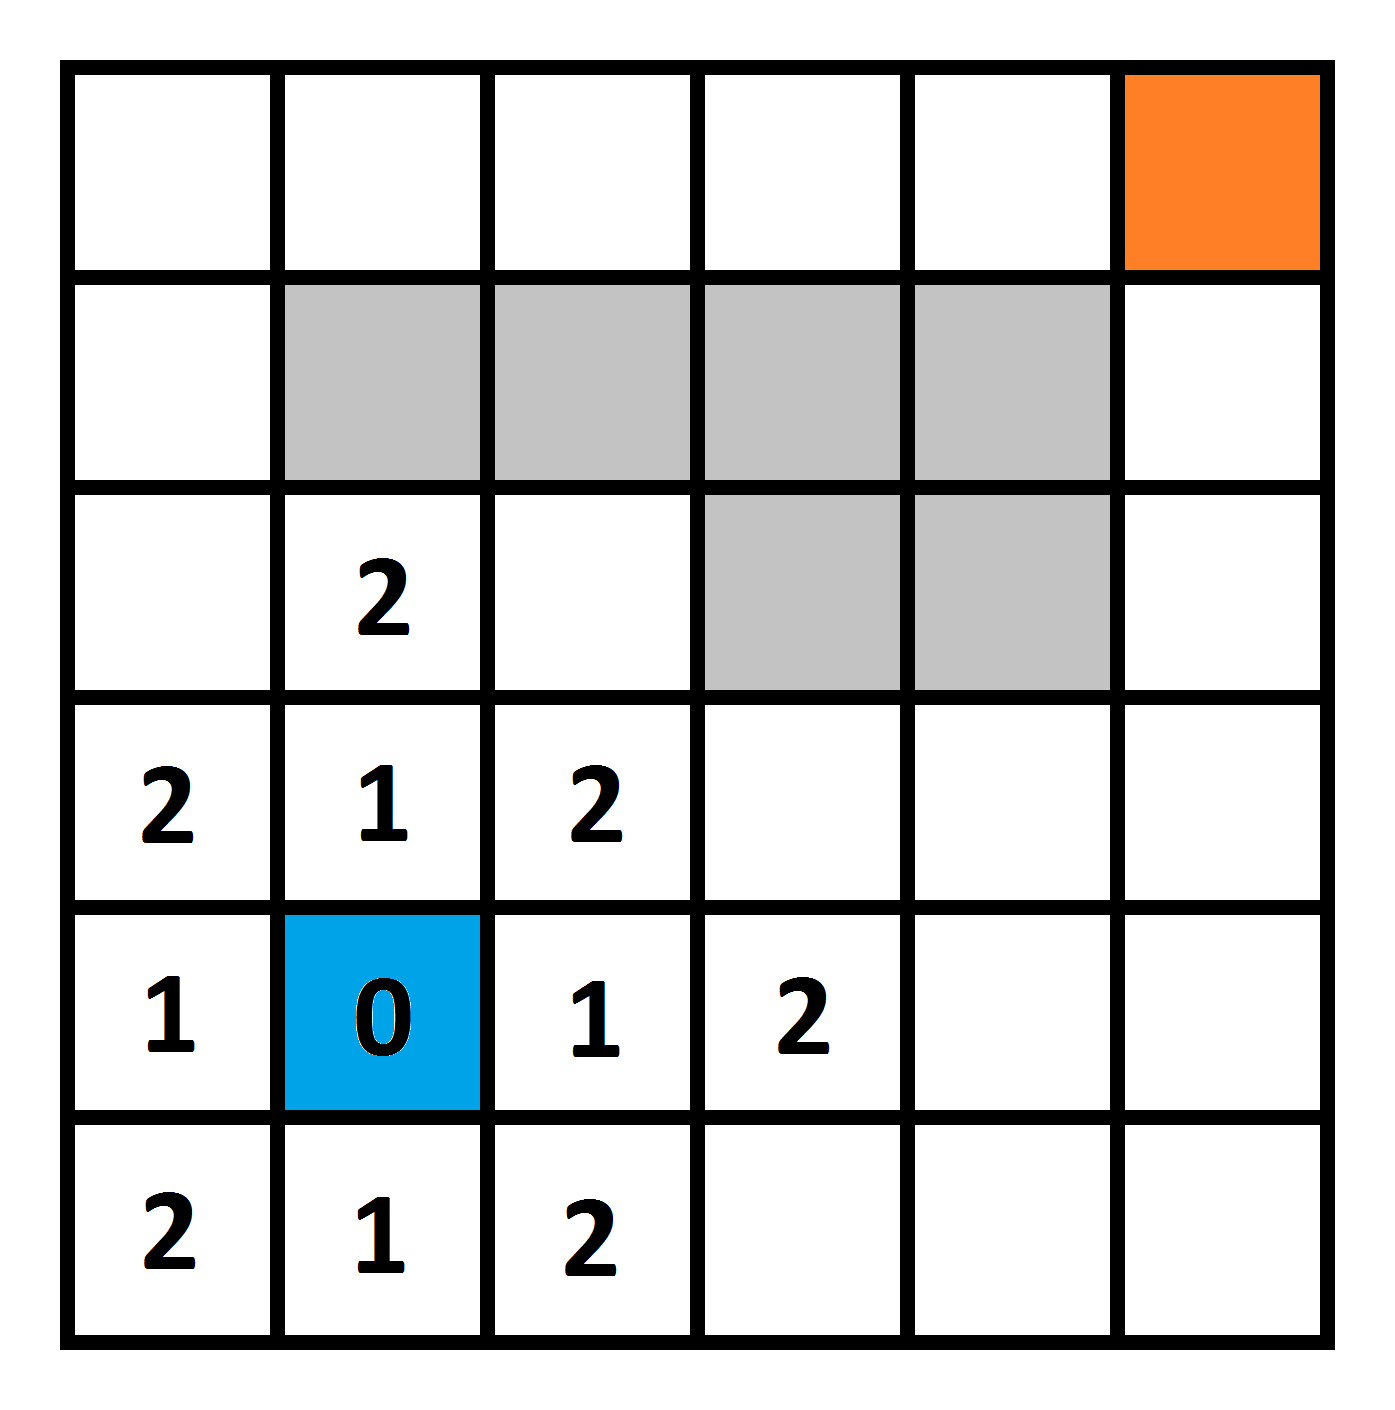
\includegraphics[width=\textwidth,height=0.8\textheight,keepaspectratio]{/FMM/grid2}	
	\end{center}
\end{frame}
\begin{frame}{Fast Marching Method}\addtocounter{framenumber}{-1}
	\begin{center}	
	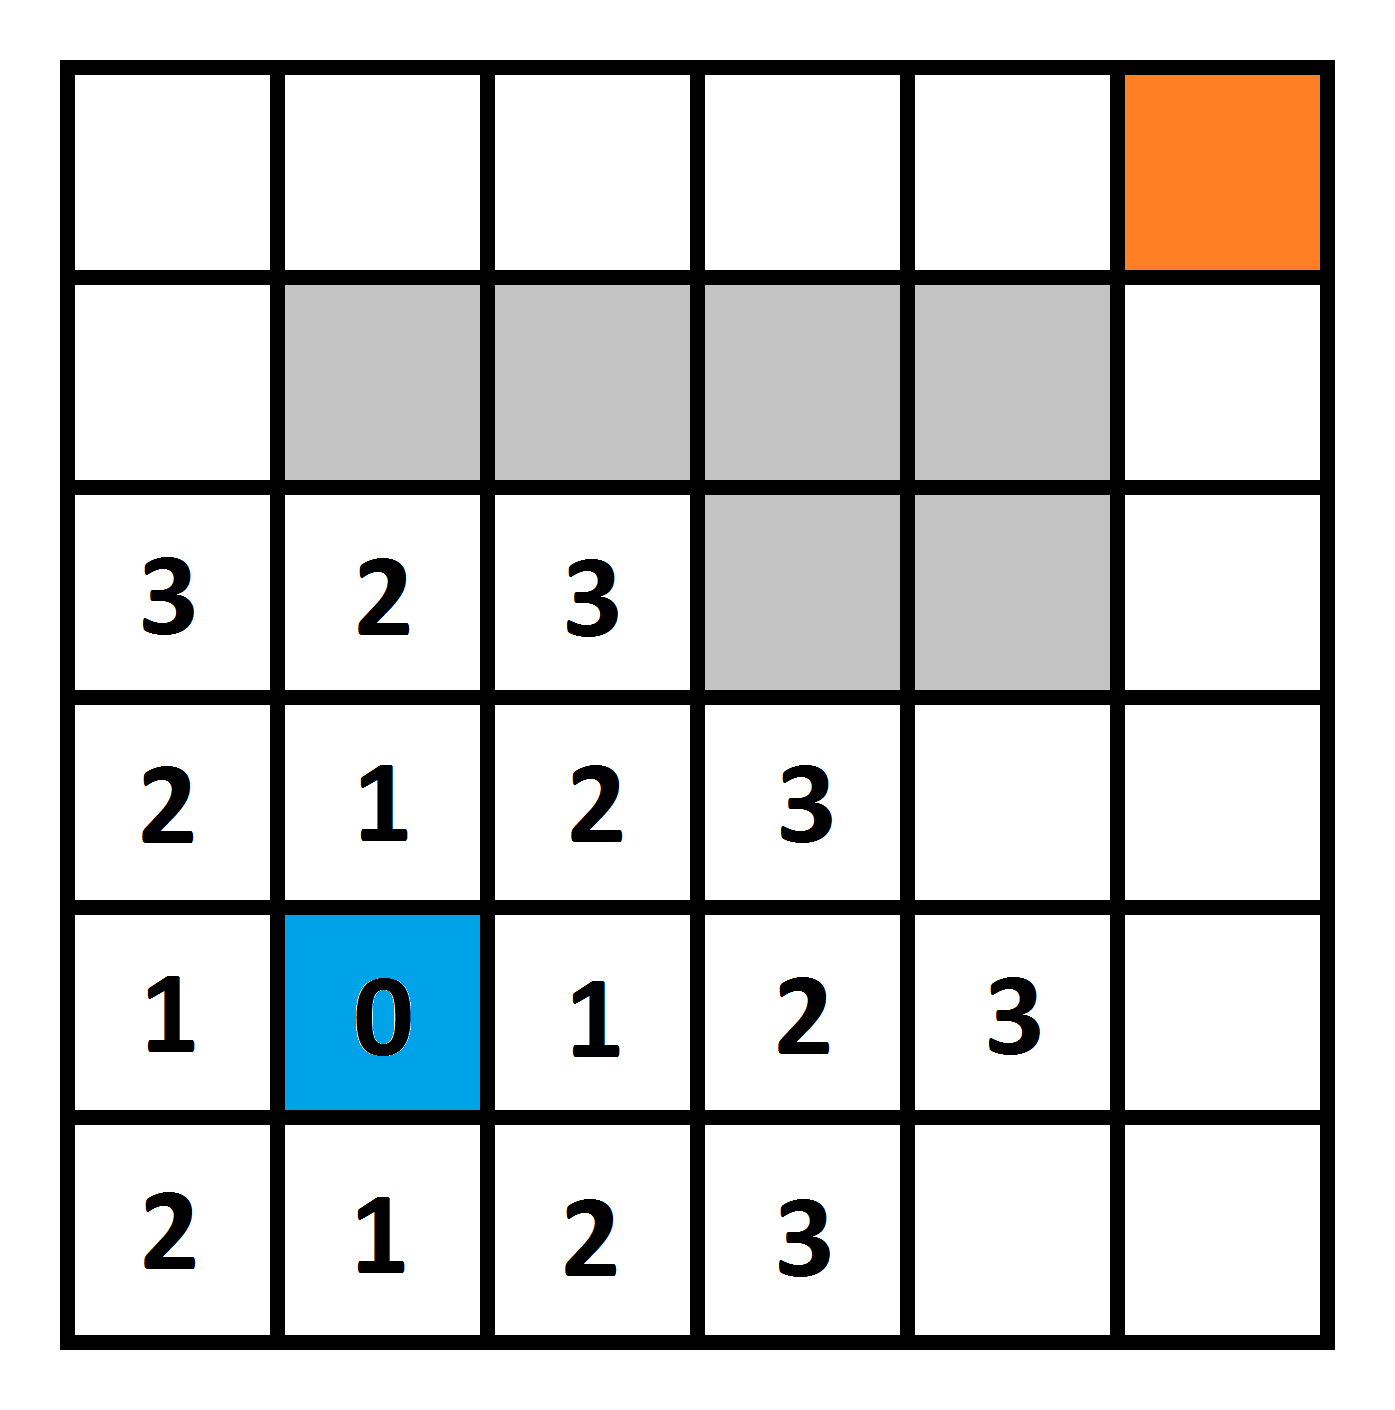
\includegraphics[width=\textwidth,height=0.8\textheight,keepaspectratio]{/FMM/grid3}	
	\end{center}
\end{frame}
\begin{frame}{Fast Marching Method}\addtocounter{framenumber}{-1}
	\begin{center}	
	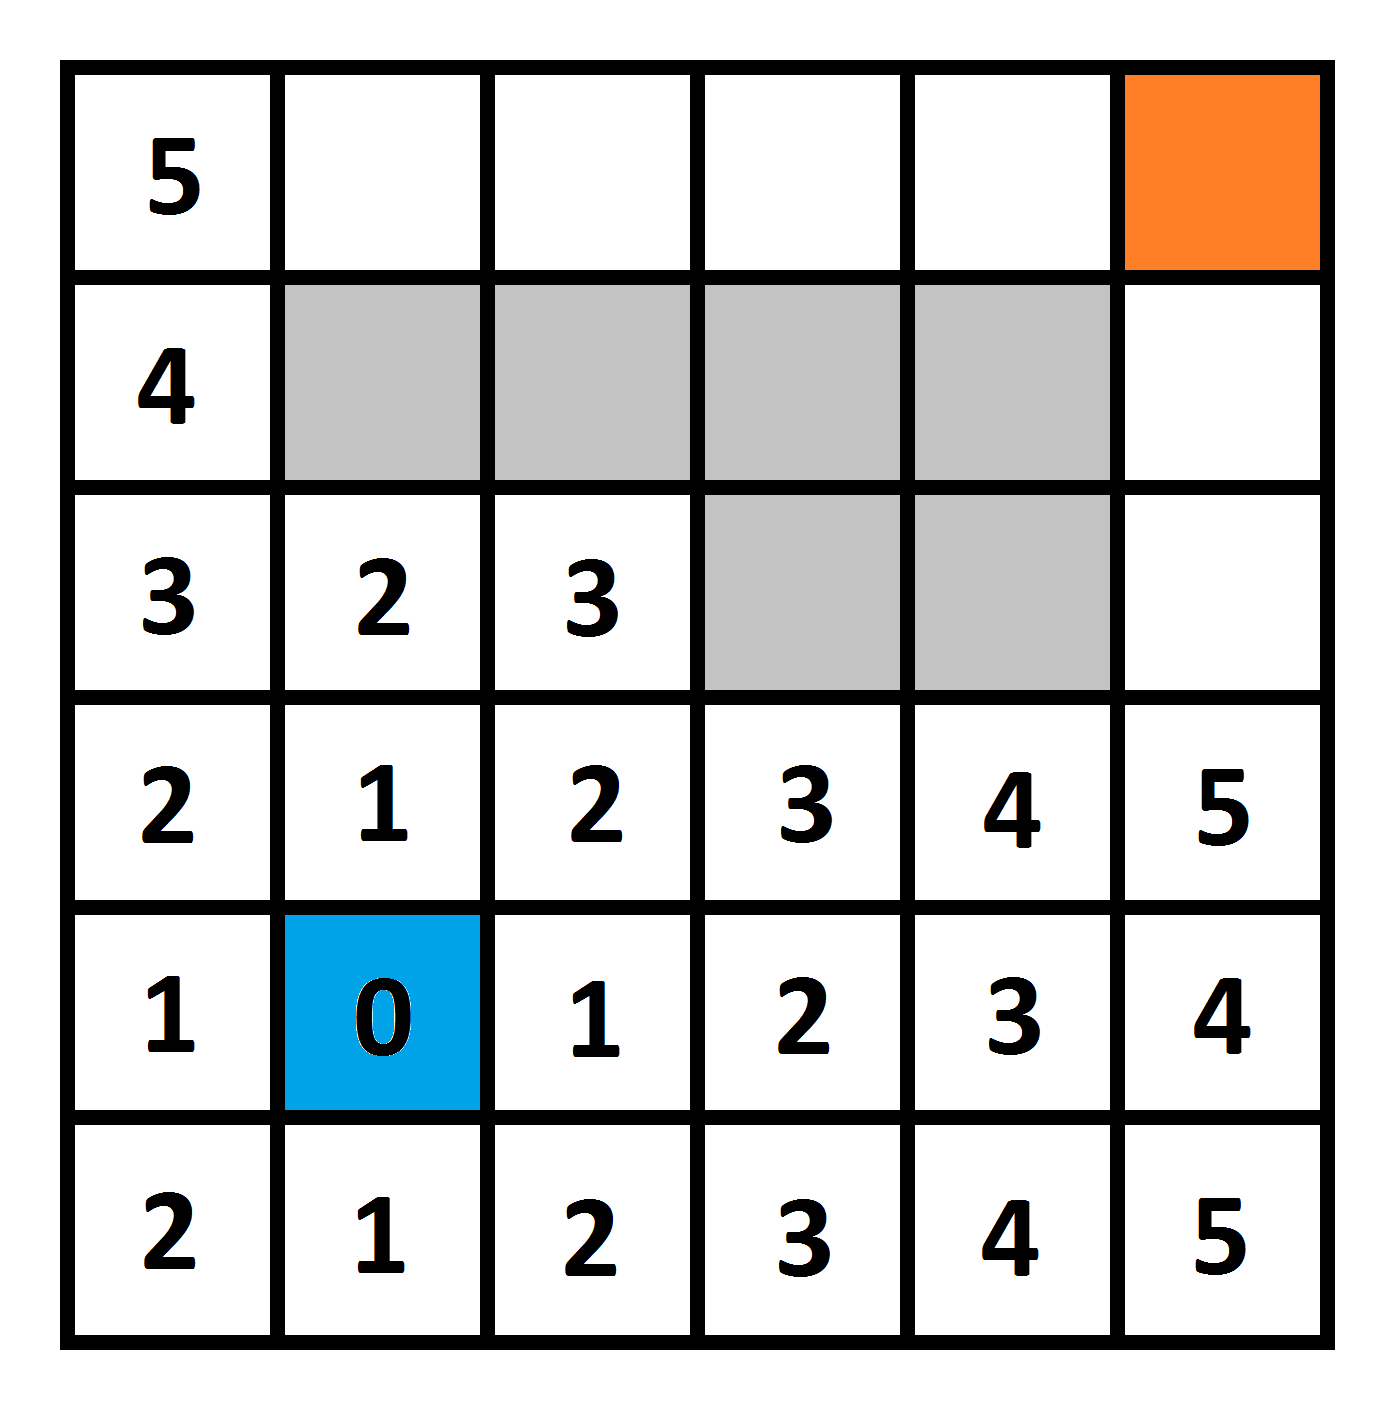
\includegraphics[width=\textwidth,height=0.8\textheight,keepaspectratio]{/FMM/grid5}	
	\end{center}
\end{frame}
\begin{frame}{Fast Marching Method}\addtocounter{framenumber}{-1}
	\begin{center}	
	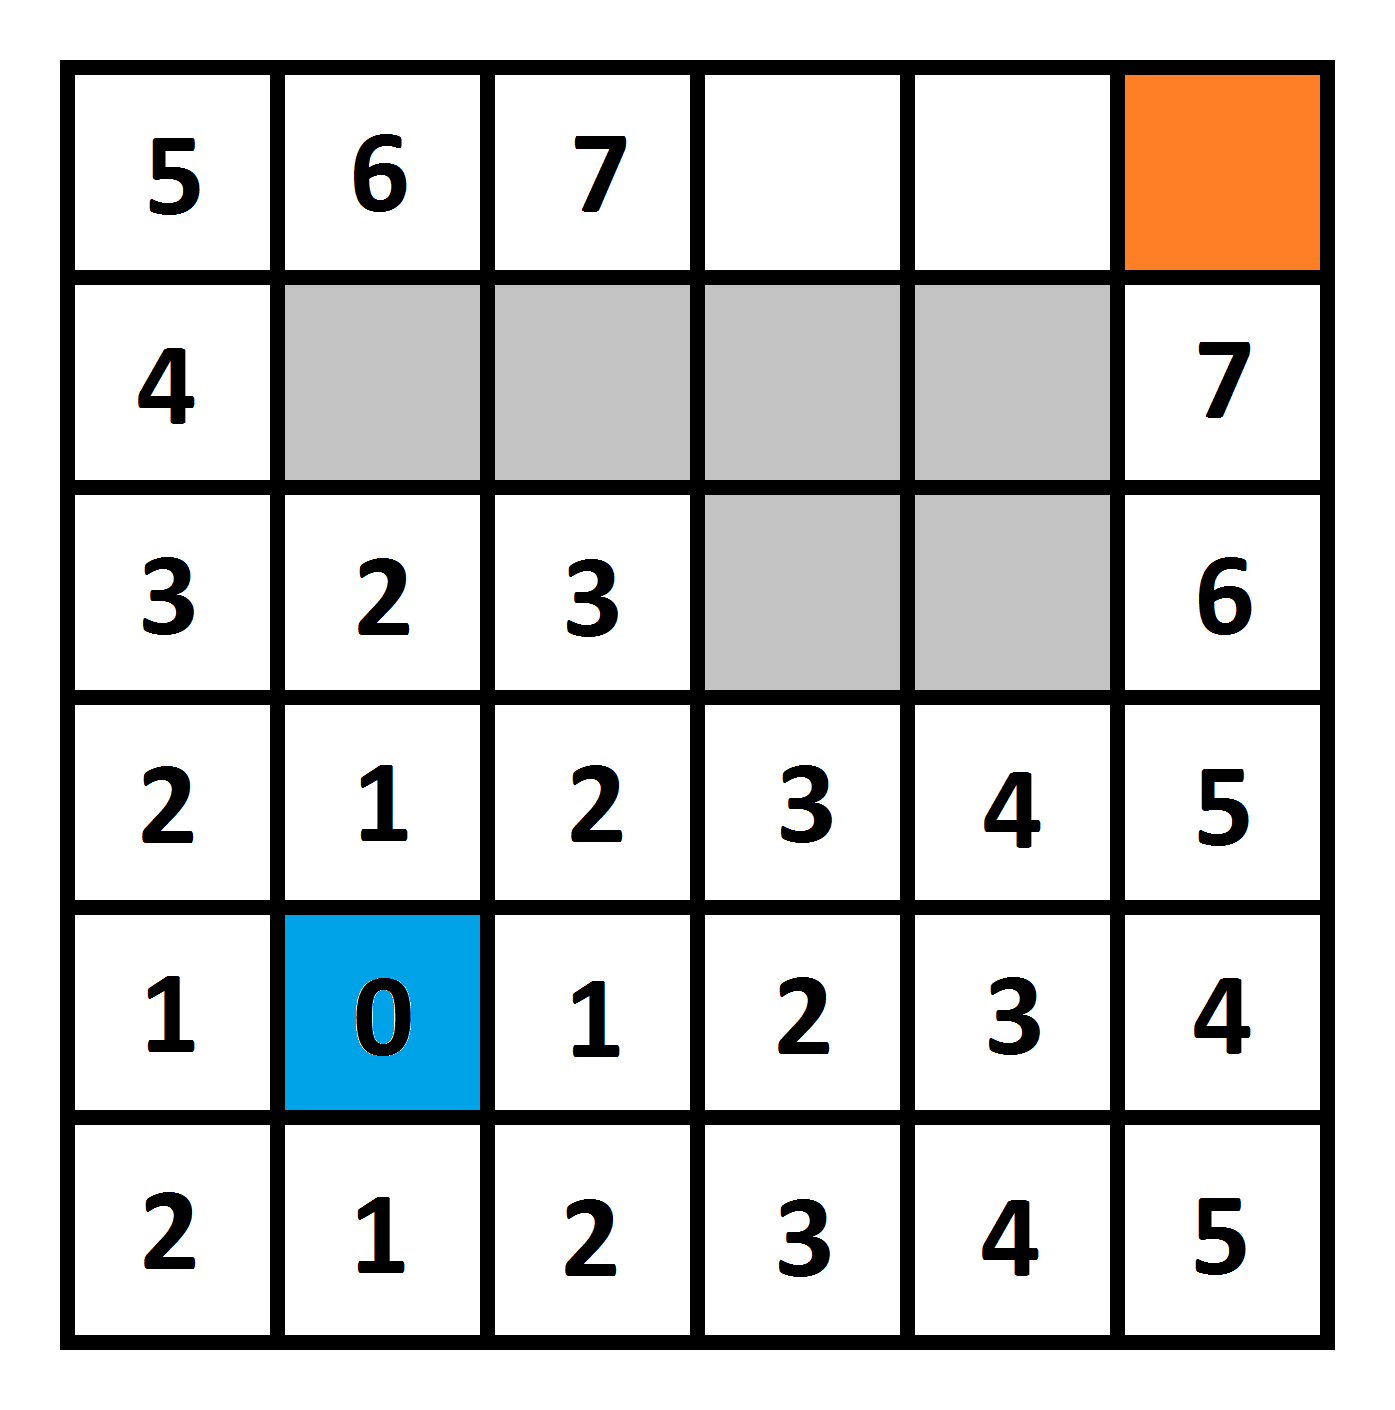
\includegraphics[width=\textwidth,height=0.8\textheight,keepaspectratio]{/FMM/grid7}	
	\end{center}
\end{frame}
\begin{frame}{Fast Marching Method}\addtocounter{framenumber}{-1}
	\begin{center}	
	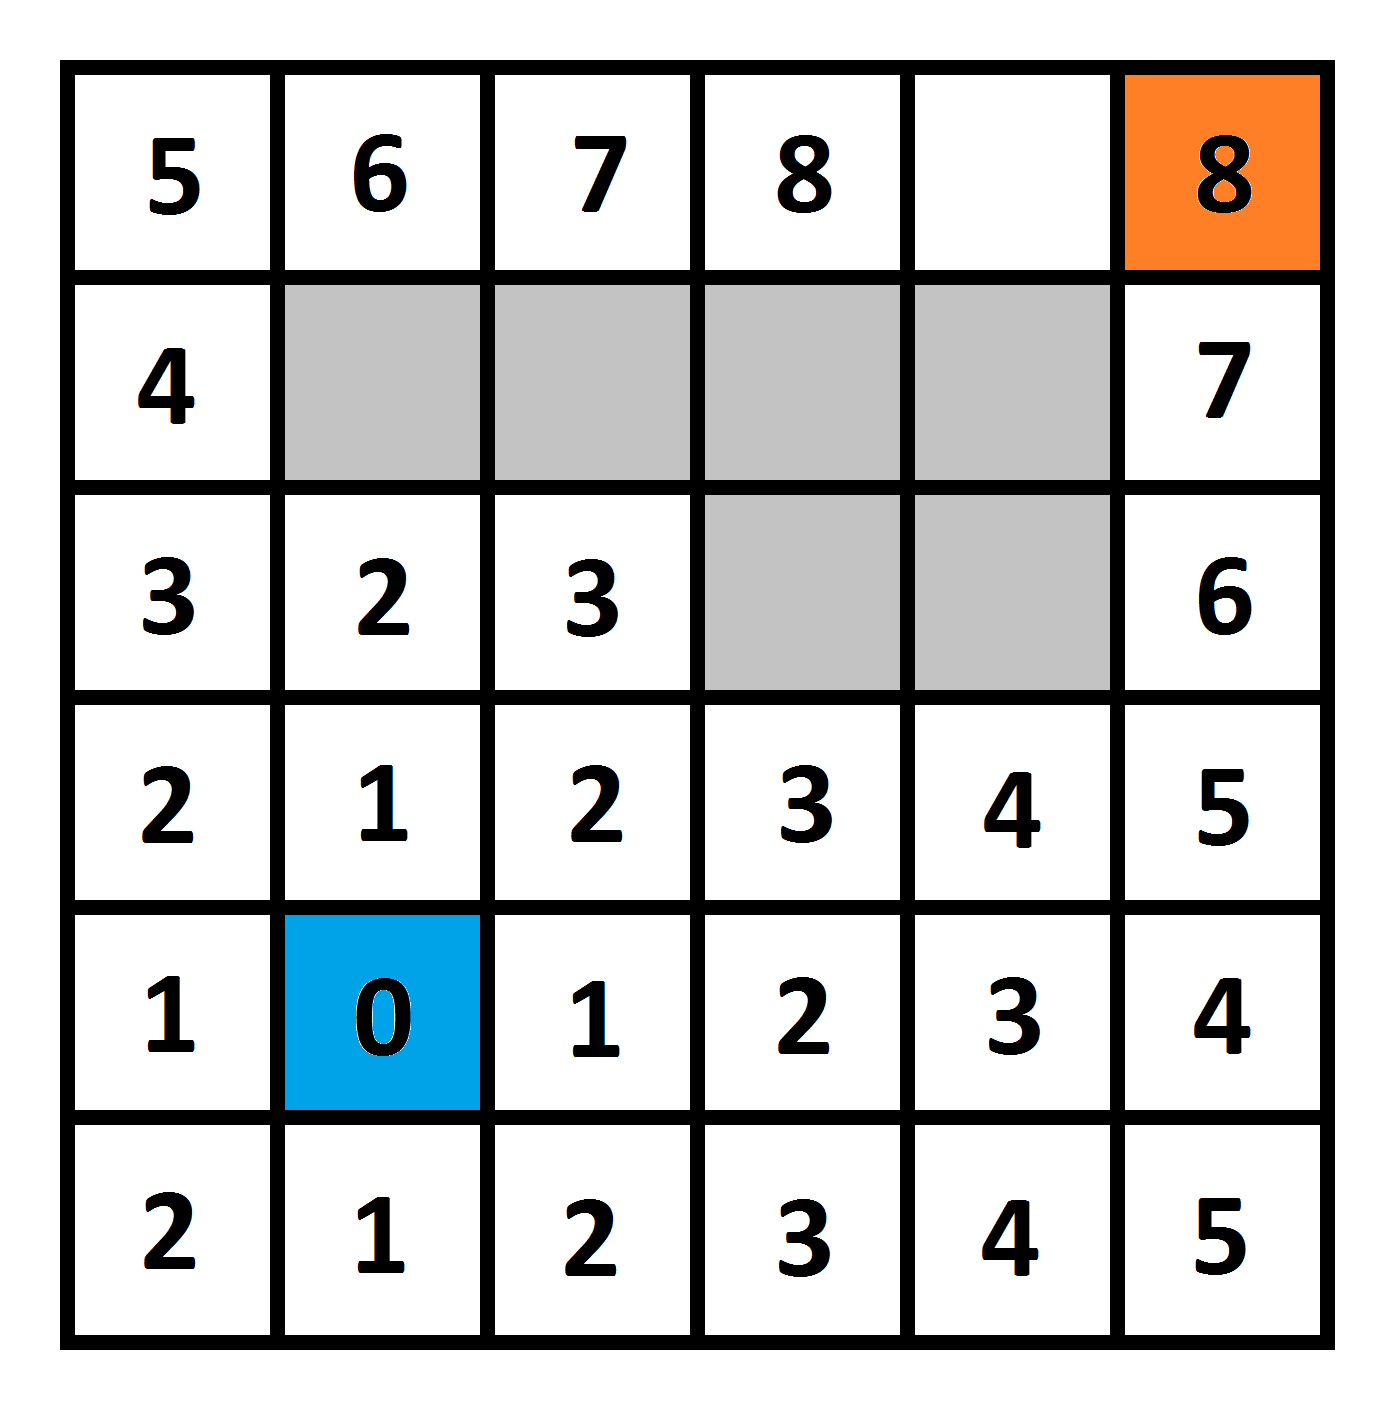
\includegraphics[width=\textwidth,height=0.8\textheight,keepaspectratio]{/FMM/grid8}	
	\end{center}
\end{frame}
\begin{frame}{Fast Marching Method}\addtocounter{framenumber}{-1}
	\begin{center}	
	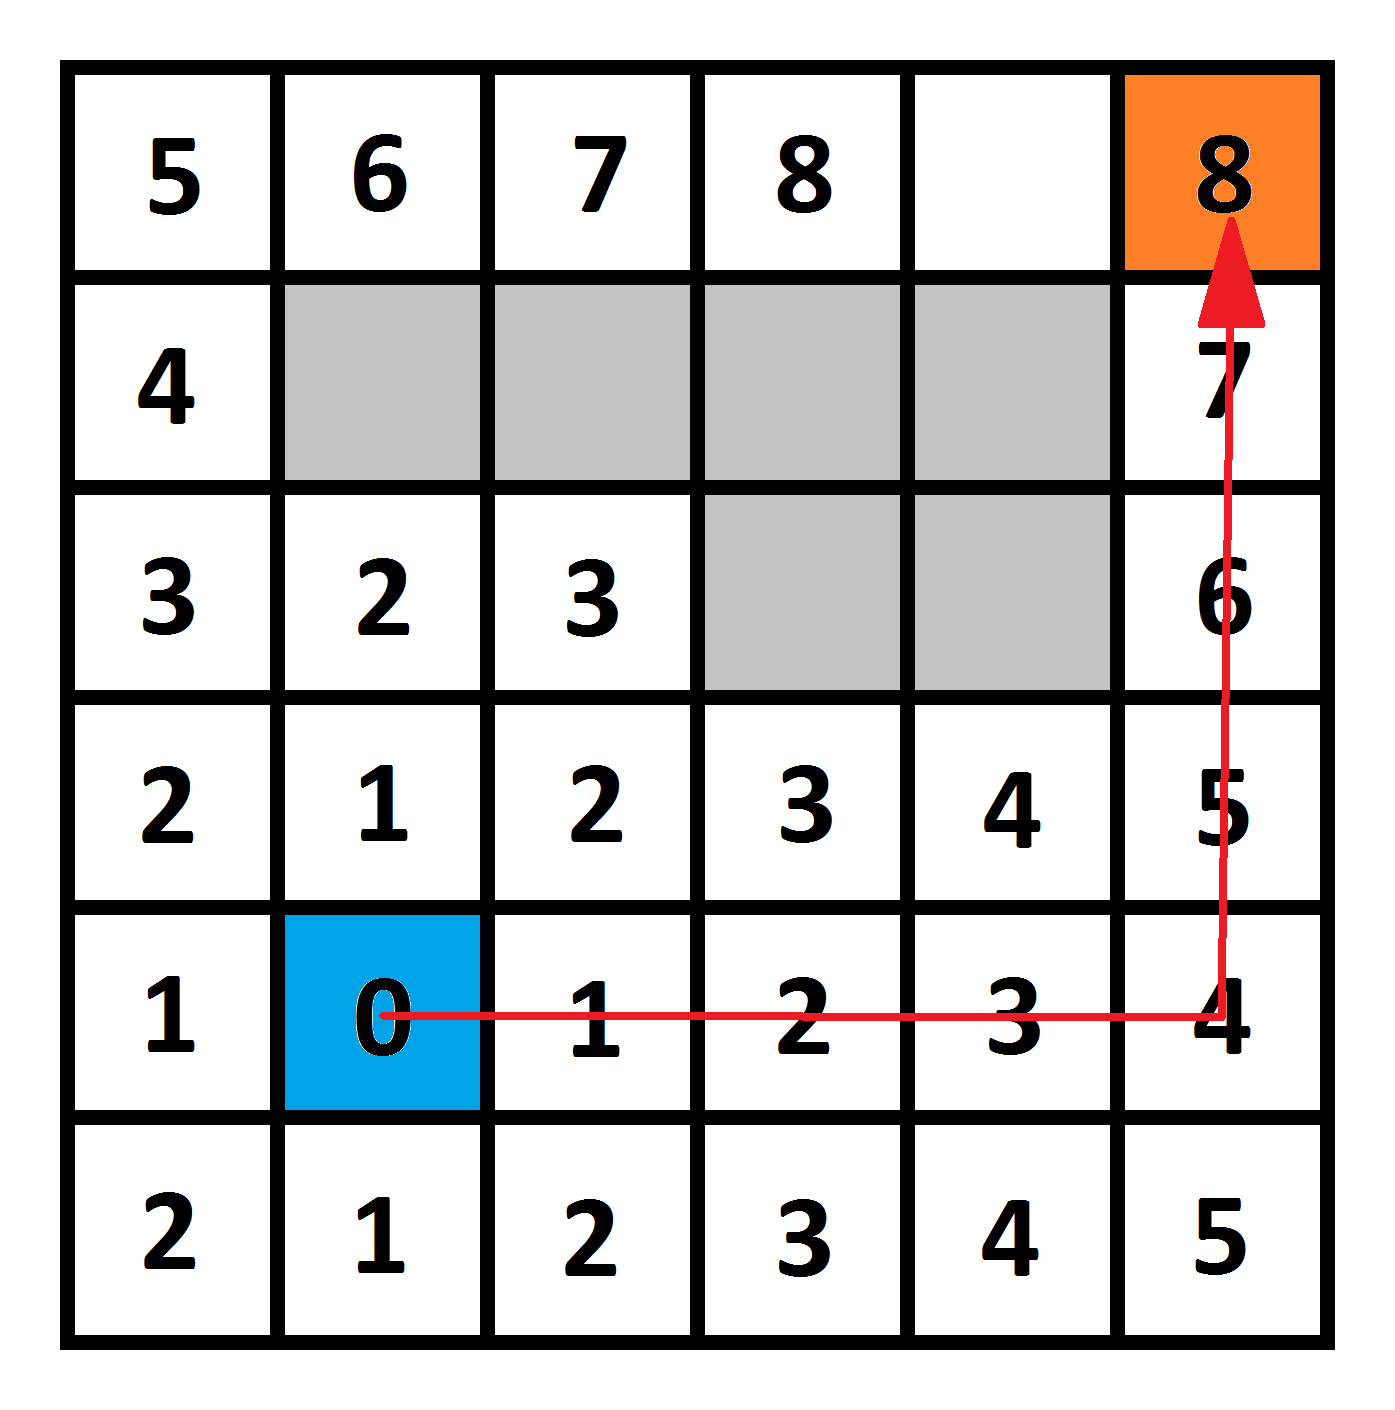
\includegraphics[width=\textwidth,height=0.8\textheight,keepaspectratio]{/FMM/gridfin}	
	\end{center}
\end{frame}

\subsection{Biblioteca nD FMM}
\begin{frame}
	Clases principales de nD FMM
	\begin{itemize}
		\item nDGridMap: Contiene la información del espacio.
		\item Solver: Implementa los algoritmos basados en FMM para la expansión de la onda.
		\item GradientDescent: Calcula el camino mediante la aplicación del descenso de gradiente.
	\end{itemize}
\end{frame}

\begin{frame}{Representación del espacio en nD FMM}
	\begin{center}	
	\includegraphics[width=0.9\textwidth,height=0.8\textheight,keepaspectratio]{grid1}	
	\end{center}
\end{frame}

%\begin{frame}{OMPL}
%Clases principales de OMPL
%\begin{itemize}
%	\item SpaceInformation
%	\item ProblemDefinition
%	\item Planner
%\end{itemize}
%\end{frame}

\begin{frame}
 \vspace{1.3cm}
	\begin{center}	
		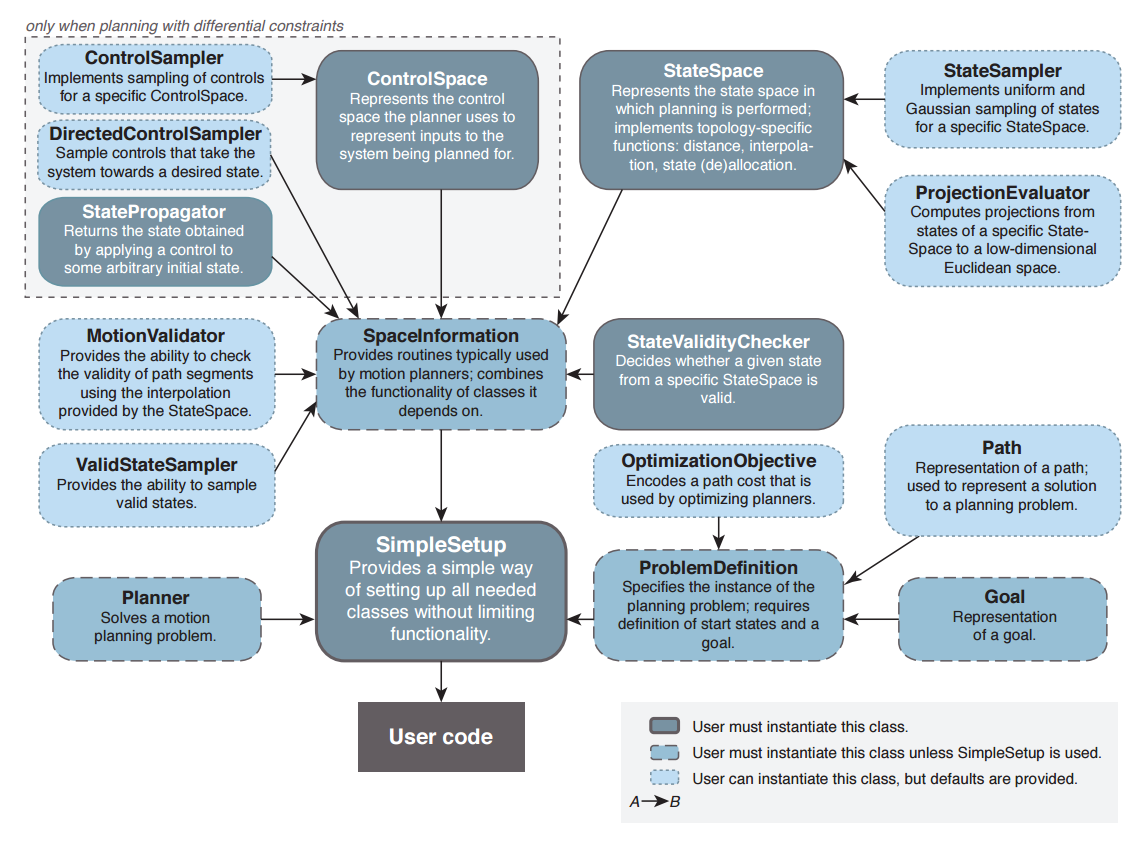
\includegraphics[width=0.8\textwidth,height=0.8\textheight,keepaspectratio]{OMPL1}	
	\end{center}
\end{frame}

\begin{frame}{Representación del espacio en OMPL}
	\begin{itemize}
		\item Describe el espacio de la manera mas general posible
		
		\item Encapsulados en clase StateSpace
			\begin{itemize}
				
				\item RealVectorStateSpace
				\item SO2StateSpace
				\item SO3StateSpace
				\item CompoundStateSpace
				\begin{itemize}
					\item SE2StateSpace
					\item SE3StateSpace
				\end{itemize}
			\end{itemize}
		\item Los espacios de estados son continuos
	\end{itemize}
\end{frame}

\begin{frame}{OMPL.app}
	\begin{itemize}
		\item Expansión de la OMPL para la resolución de problemas SE(2) y SE(3)
		\item SE2RigidBodyPlanning y SE3RigidBodyPlanning
		\item Implementa un detector de colisiones
		\item Permite cargar archivos COLLADA de entornos y robots en 3D
		\item Incluye una interfaz gráfica de usuario	
		
	\end{itemize}
\end{frame}


\section{Trabajo Realizado}

\begin{frame}{Conversión de estados}
	\begin{multicols}{2}
		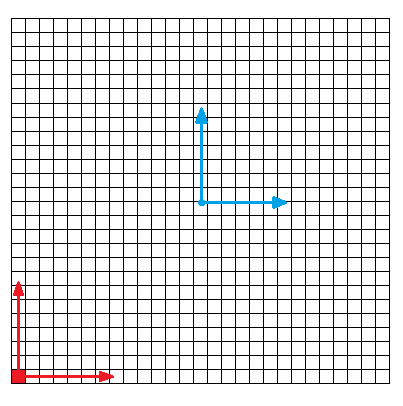
\includegraphics[width=0.45\textwidth,keepaspectratio]{ejes}	
		\begin{enumerate}
			\item Utilizar método \textit{as<T>} para hacer casting de StateSpace
			\item Obtener vector de coordenadas
			\item Obtener límites del entorno
			\item Unificar ejes de coordenadas
			\item Convertir coordenadas a índice en la rejilla
		\end{enumerate}
	\end{multicols}
\end{frame}

\subsection{Rotacion}
\begin{frame}{Conversión de la rotación}
	\begin{center}
	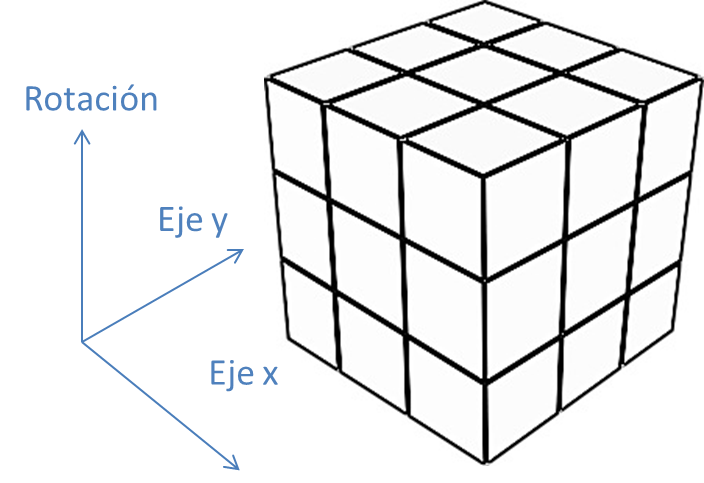
\includegraphics[width=0.7\textwidth,height=0.6\textheight,keepaspectratio]{rotacion}	
	\end{center}
\end{frame}

\begin{frame}{Conversión de mapas de OMPL a nD FMM}
	\begin{itemize}
		\item No todos los algoritmos requieren mapas exactos
		\item Es preferible en algunos casos minimizar el coste computacional
		
		\vspace{0.5cm}
		\item Dos tipos de métodos para convertir mapas
			\begin{itemize}
				\item Muestreo secuencial
				\item Muestreo aleatorio
			\end{itemize}
		
	\end{itemize}
\end{frame}

\begin{frame}{Métodos aleatorios}
\begin{center}
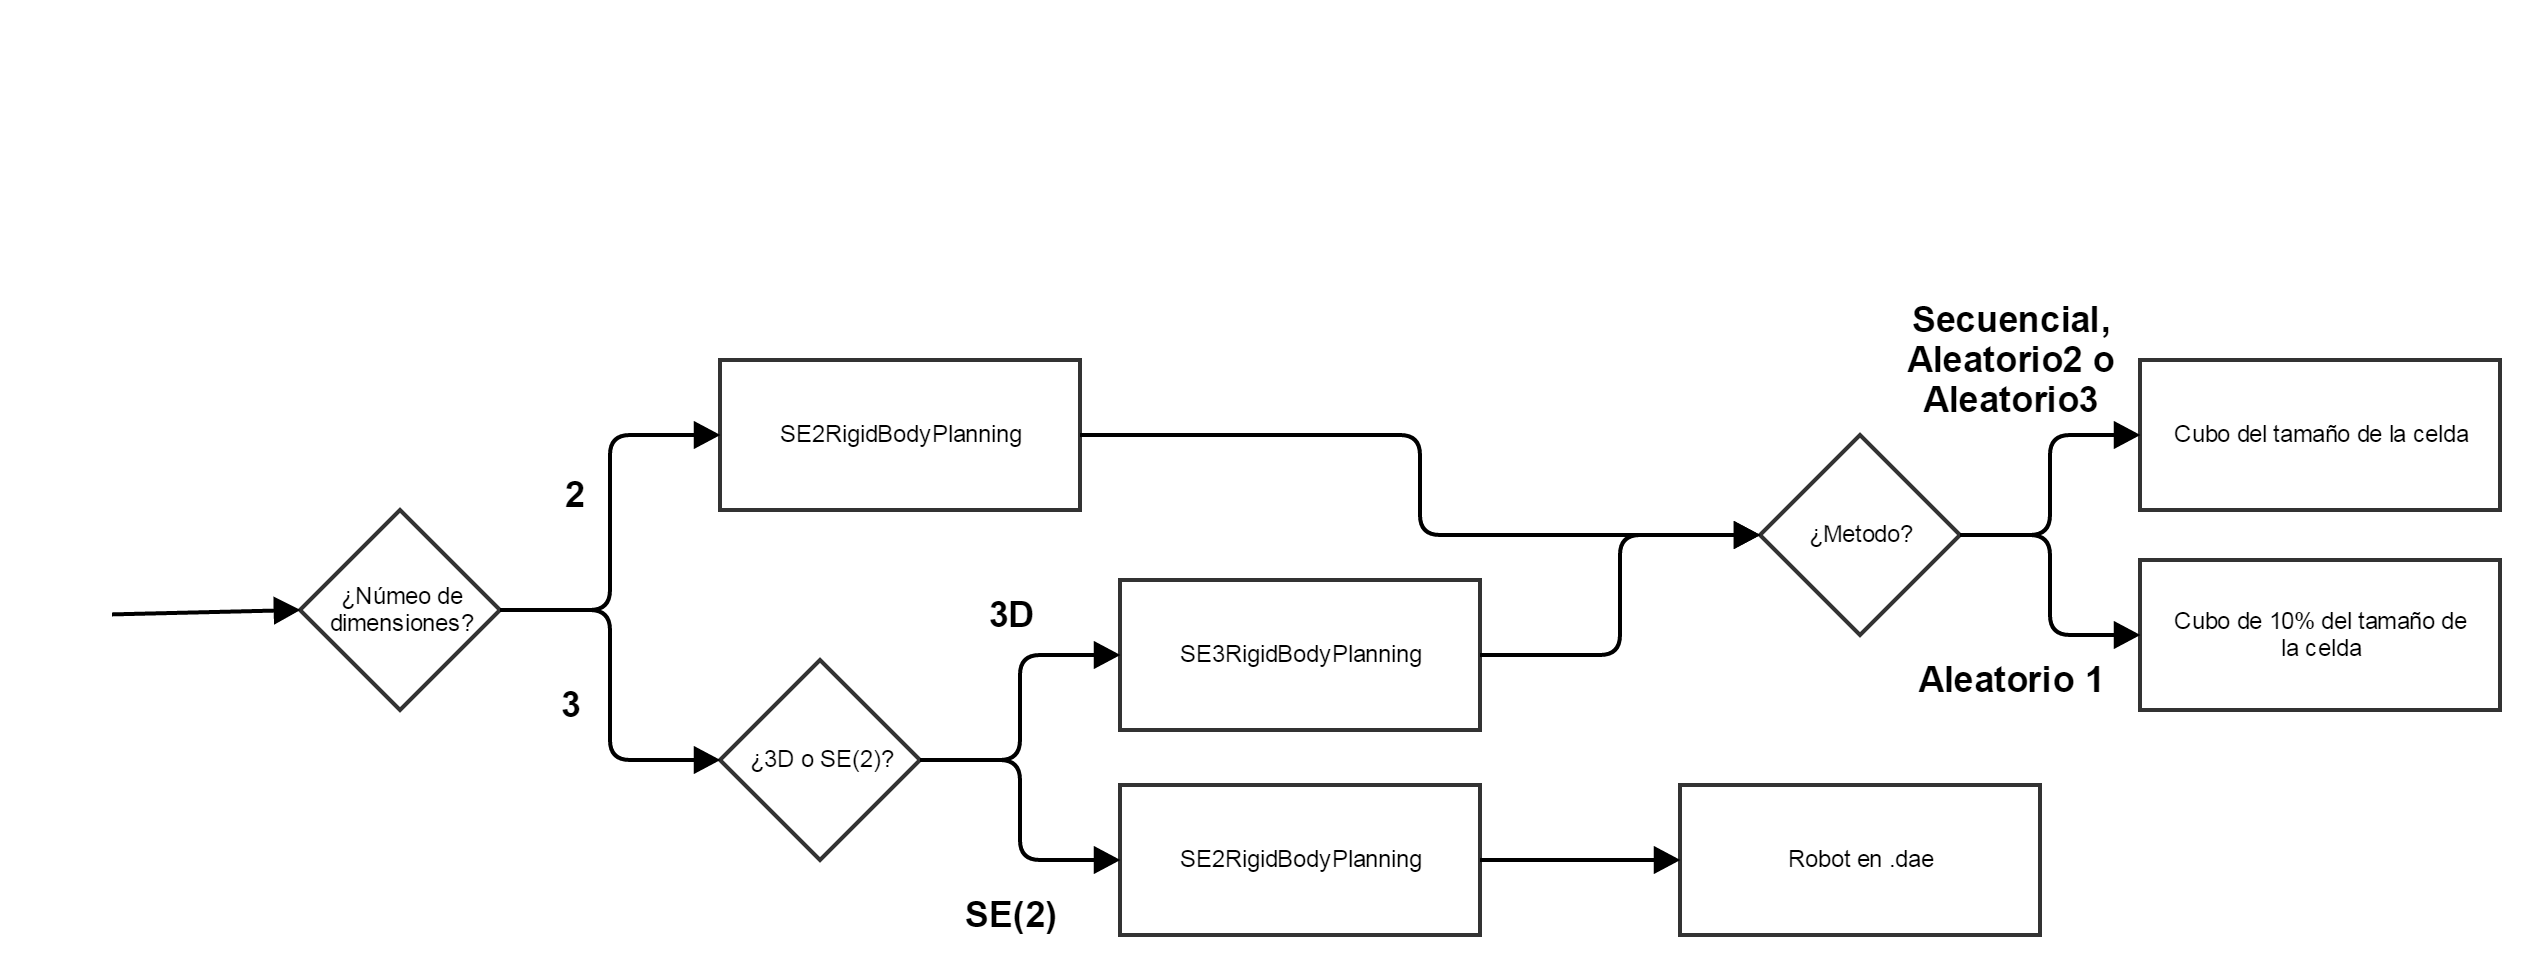
\includegraphics[width=\textwidth,height=0.8\textheight,keepaspectratio]{seleccion}	
\end{center}
\end{frame}

\begin{frame}{Comparación de métodos 1 y 2}
\begin{center}
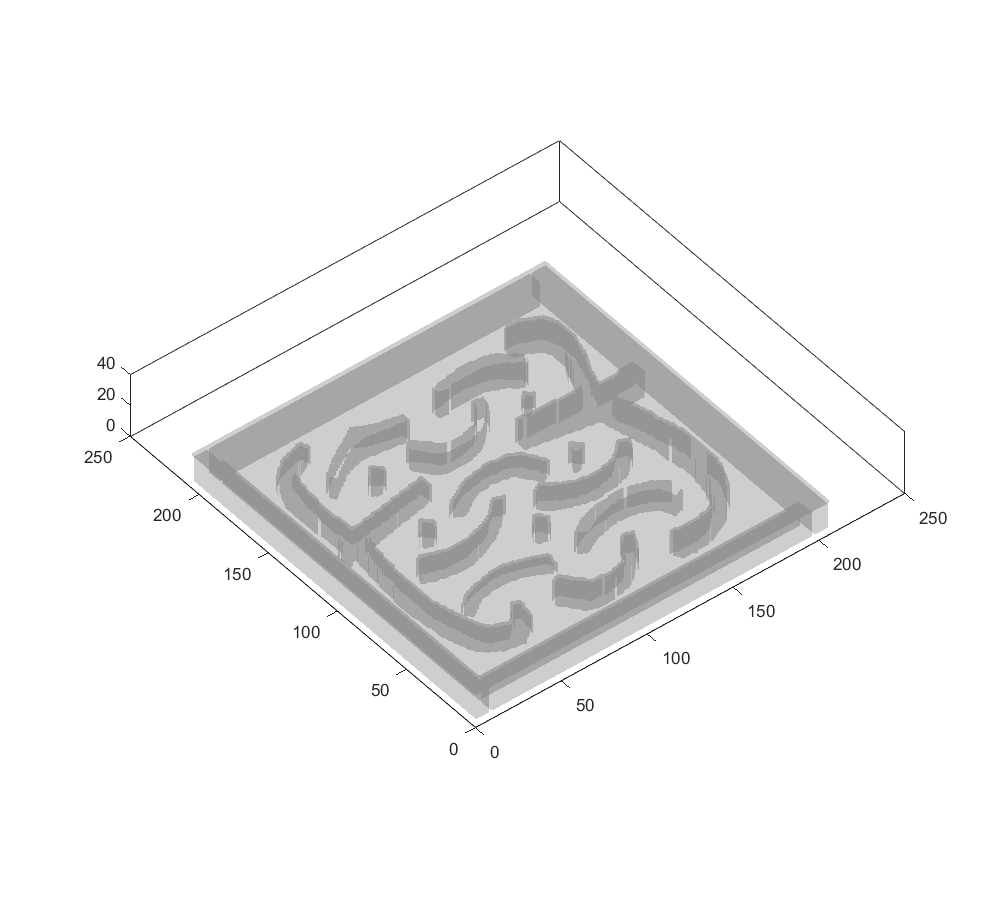
\includegraphics[width=0.38\textwidth]{/Tests/MazeN7M03D}
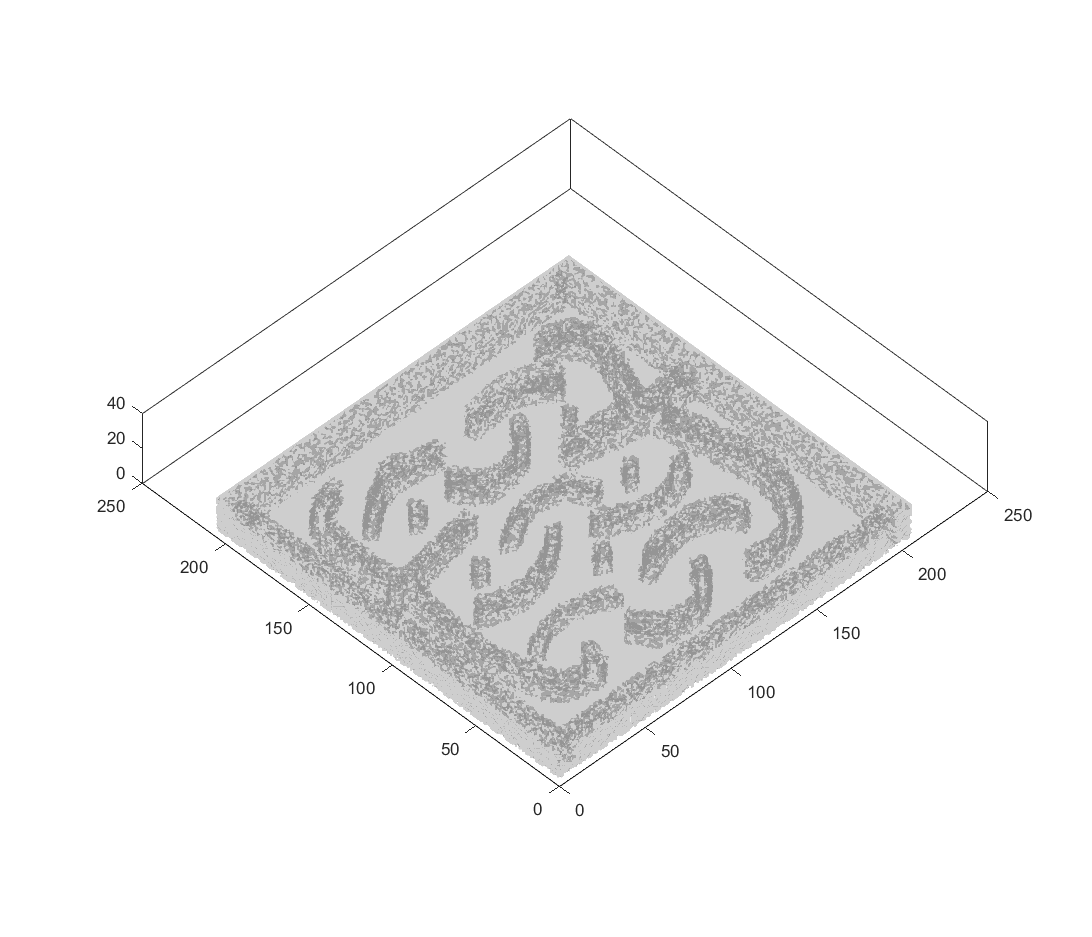
\includegraphics[width=0.38\textwidth]{/Tests/MazeN5M1P033D}

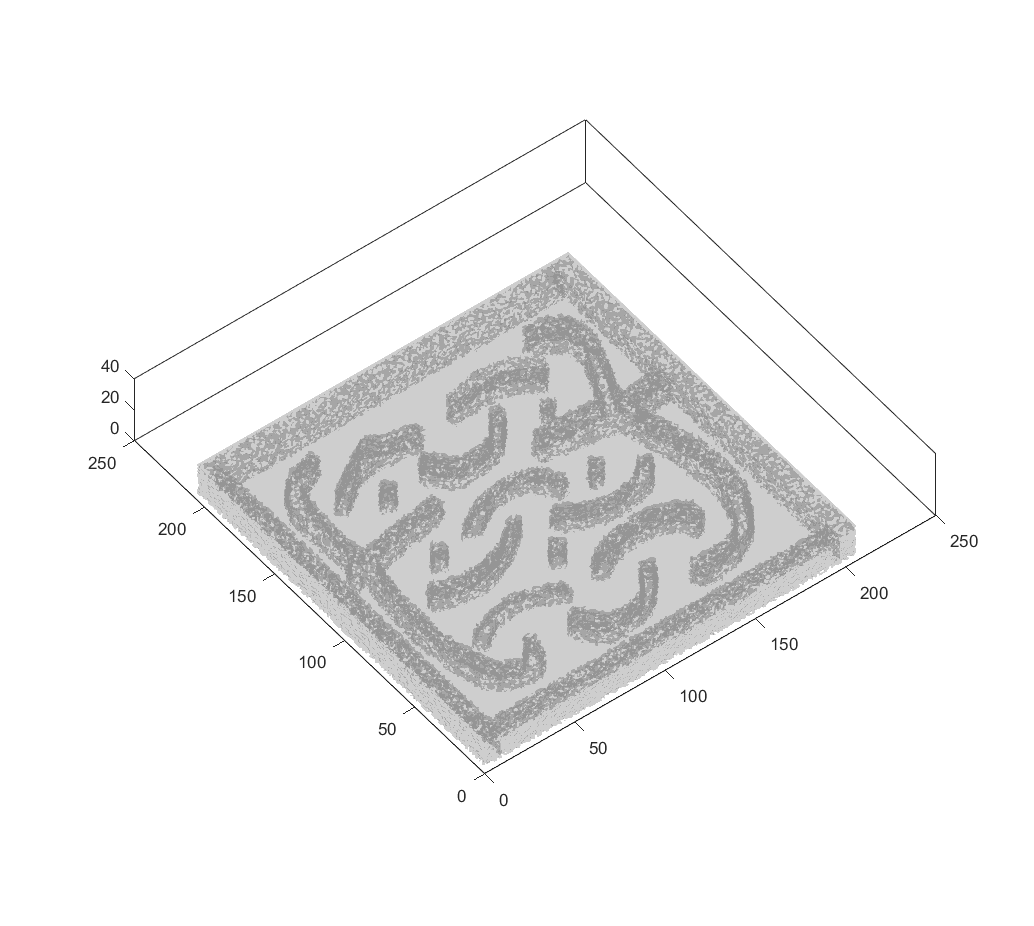
\includegraphics[width=0.38\textwidth]{/Tests/MazeN5M1P093D}
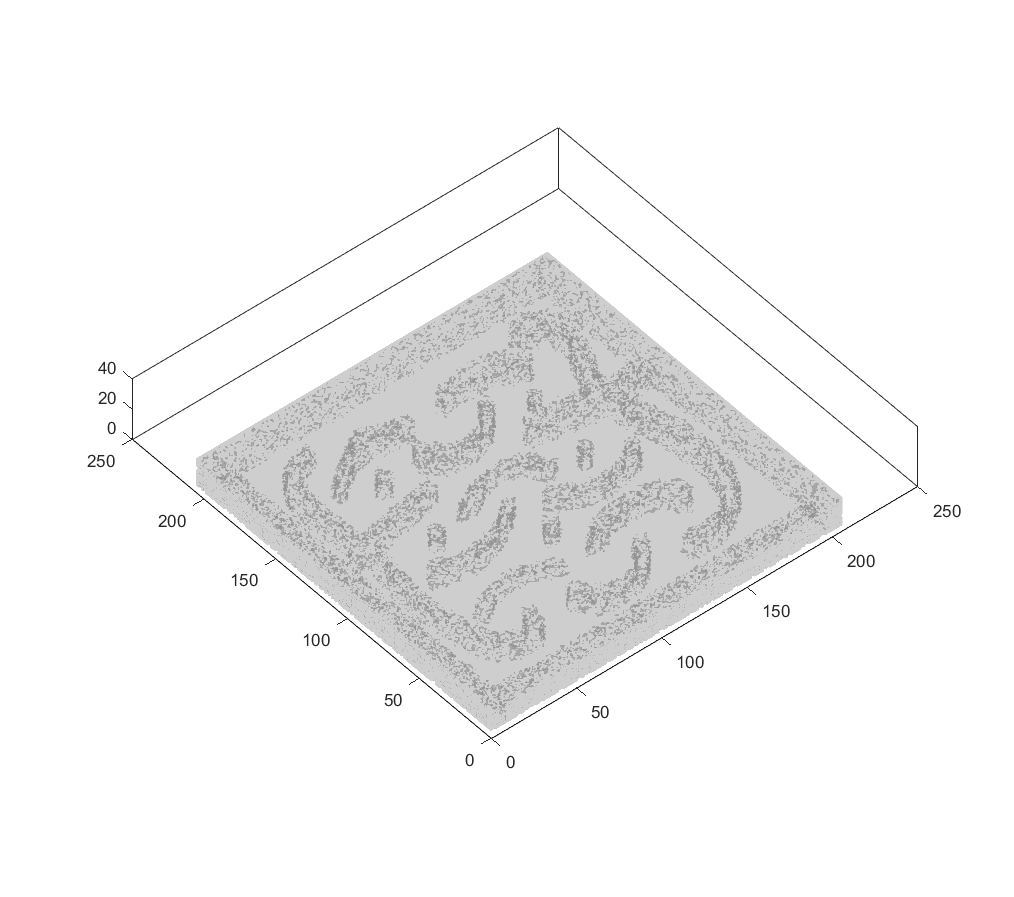
\includegraphics[width=0.38\textwidth]{/Tests/MazeN6M1P033D}
\end{center}
\end{frame}

\begin{frame}{Comparación de métodos 1 y 2}
\vfill
\begin{center}
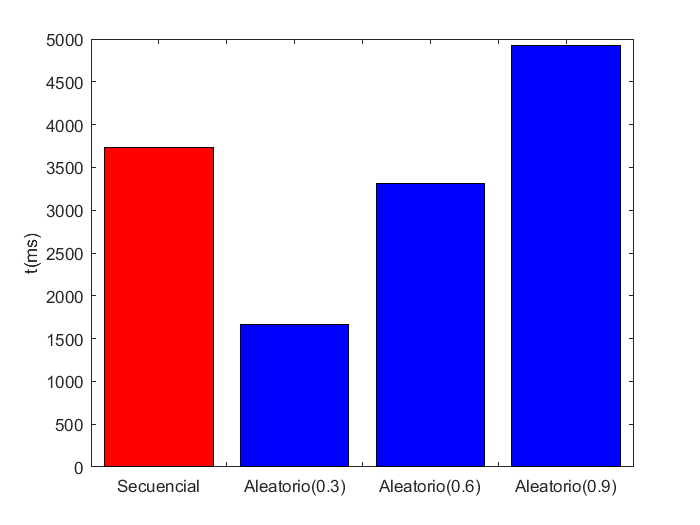
\includegraphics[width=0.7\textwidth]{/Tests/T13D}
\end{center}
\end{frame}

\section{Resultados y conclusiones}

\begin{frame}{Video example}
\begin{center}
\includemedia[
    width=6cm,height=6cm,
    activate=pageopen,
    addresource=vid.flv,
    flashvars={
        source=vid.flv
       &autoPlay=true
    }
]{}{VPlayer.swf}
\end{center}
\end{frame}


{\aauwavesbg
	\begin{frame}[plain,noframenumbering]
		\finalpage{¿Alguna pregunta?}
	\end{frame}}

\end{document}
